\Testart{Skript}
\Klasse{10}
\Fach{Informatik}
\Titel{Datenbanken}

\renewcommand{\Content}{
    
    \mysession{Stunde 1+2}{
        \input{_Hefteintraege/H00_KlassenObjekte}

        \input{_Aufgaben/A00_Objektkartenmemory}
    }
    \mysession{Stunde 3+4}{
        \input{_Aufgaben/A01_KlasseZurTabelle}

        \input{_Hefteintraege/H01_AufbauDB}

        \input{_Hefteintraege/H02_Spickzettel}

        \input{_Aufgaben/A02_SQLIsland}

    }
    \mysession{Stunde 5+6}{

        \input{_Aufgaben/A03_SQL-Puzzle}

        \input{_Aufgaben/A04_SQL-Basics}
    }
        
    \mysession{Stunde 7+8}{
        \input{_Aufgaben/A05_ErarbeitungBeziehungen}
    
        \Hefteintrag{1.8}{Tabellenbeziehungen: Fremdschlüssel}{
	Wenn Datensätze mittels Primärschlüssel in einer anderen Tabelle verwendet werden, spricht man dort von einem Fremdschlüssel. Im \emphColA{Tabellenschema} werden die \emphColA{\LoesungLuecke{Fremdschlüssel}{8cm}} durch \emphColA{\ifloesung $\overline{\text{\textbf{überstreichen}}}$ \else $\overline{\text{\textbf{~~~~~~~~~~~~~~~~~~~~~~~~~~~~~~~~~~~~~~~~~~~~~~~~~~~~~~~~~~~~~~~~~}}}$ \fi} (manchmal auch \emphColA{\ifloesung \dotuline{unterpunkten} \else \dotuline{~~~~~~~~~~~~~~~~~~~~~~~~~~~~~~~~~~~~~~~~~~~~~~~~~~~~~~~~~~~~} \fi}) markiert. Ein Beispiel in SQL-Island ist der Häuptling eines Dorfes, der in der Tabelle Dorf mittels bewohnernr eingetragen wird. Die \emphColB{bewohnernr} ist hierbei \emphColB{\LoesungLuecke{Primärschlüssel}{8cm}} in der \emphColB{Tabelle Bewohner} und \emphColC{\LoesungLuecke{Fremdschlüssel}{8cm}} in der \emphColC{Tabelle Dorf} (heißt hier aber \emphColC{haeuptling}).

}



        \input{_Hefteintraege/H04_BeziehungKlassendiagramm}

        \input{_Hefteintraege/H05_Kardinalität}

        \input{_Aufgaben/A06_Flugverspaetung}
    }
        
    \mysession{Stunde 9+10}{

        \ifbeamer
        \input{_Aufgaben/A06_Flugverspaetung}
        \fi

        \input{_Aufgaben/A07_ErarbeitungKreuzprodukt}

        \input{_Hefteintraege/H06_Kreuzprodukt}
        
        \input{_Hefteintraege/H07_KreuzproduktBeispiel}
    }
    
    \mysession{Stunde 11+12}{
        \ifbeamer
            \input{_Hefteintraege/H07_KreuzproduktBeispiel}
        \fi
        \input{_Aufgaben/A08_KreuzproduktJoin_Bayern}
    }

    \mysession{Stunde 13 bis 16}{

        \Aufgabe{Zwei Diagramme für eine Datenbank?}{
Folgende Diagramme stellen dieselbe Datenbank dar. 
Finde Unterschiede und erkläre wieso sie auftreten. Nutze bei Bedarf auch 
\UrlAndCode{www.dbiu.de/bayern/}

\vspace{0.3cm}

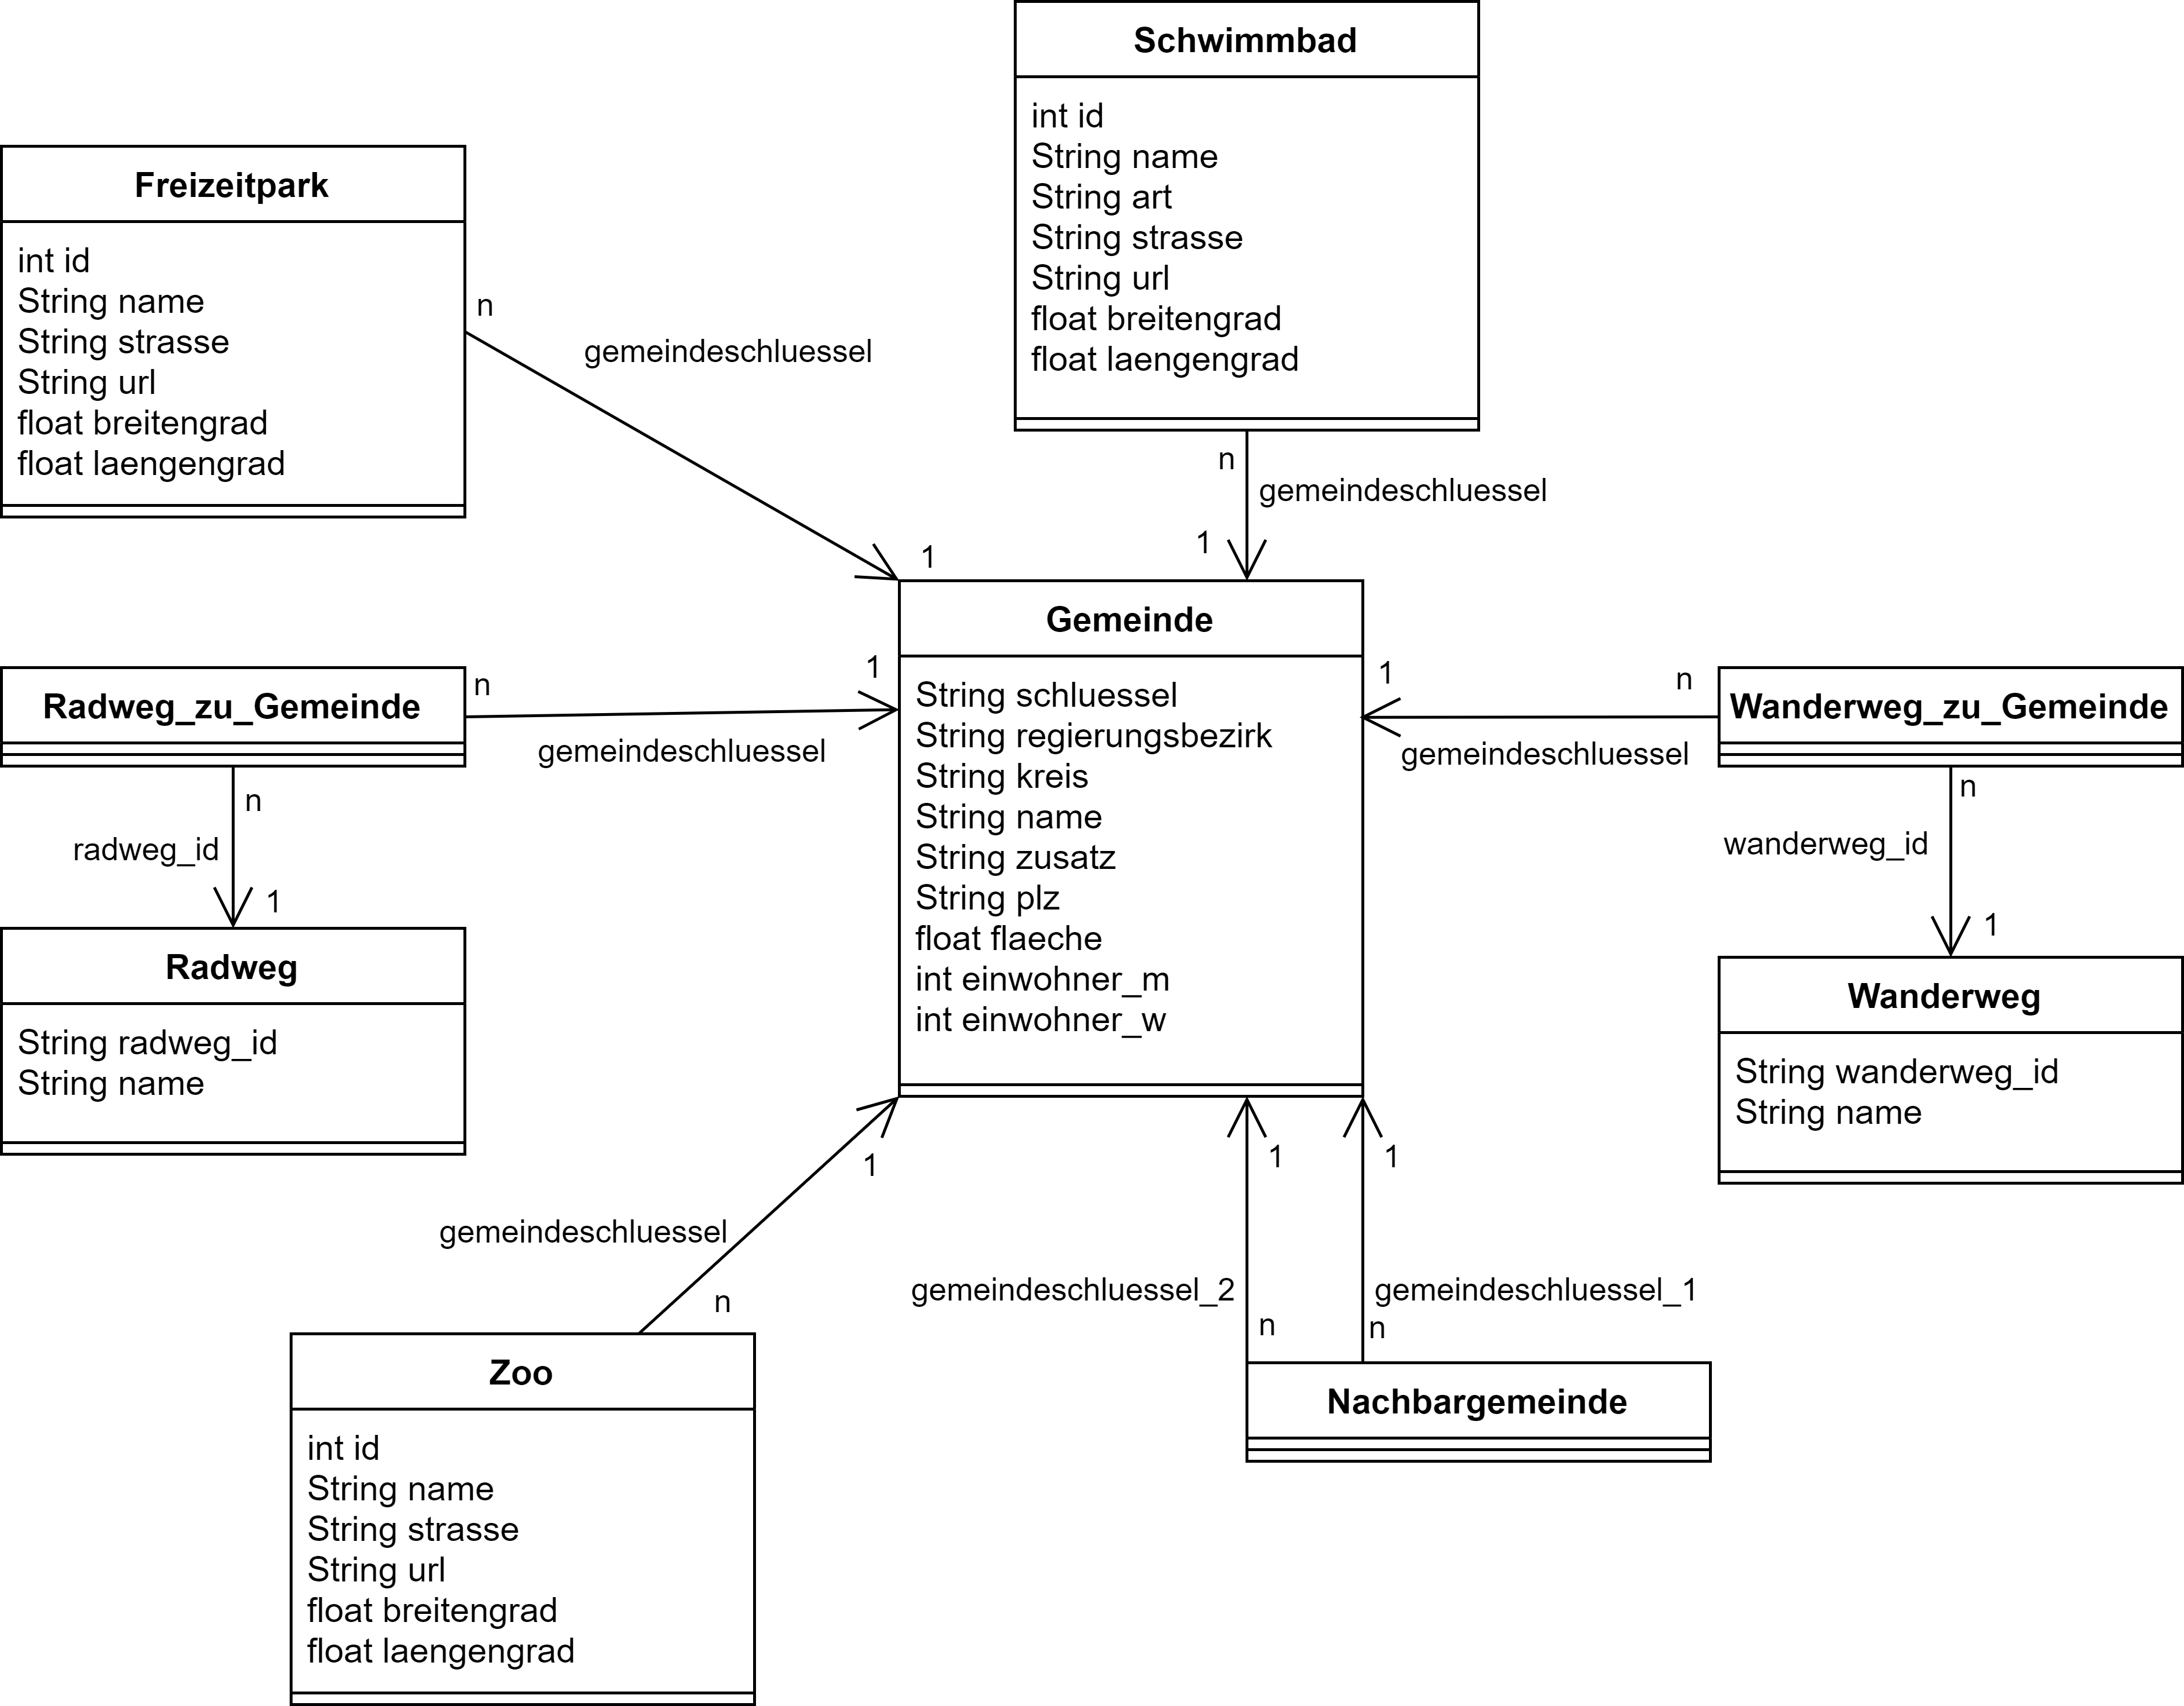
\includegraphics[width=0.92\textwidth]{_Aufgaben/img/A09_Bayern_DB.png}

\vspace{1cm}

\begin{tikzpicture}
    \begin{class}{Gemeinde}{0,0}
        \attribute{String schluessel}
        \attribute{String regierungsbezirk}
        \attribute{String kreis}
        \attribute{String name}
        \attribute{String zusatz}
        \attribute{String plz}
        \attribute{float flaeche}
        \attribute{int einwohner$\_$m}
        \attribute{int einwohner$\_$w}
    \end{class}
    \begin{class}{Freizeitpark}{-6.5,3}
        \attribute{int id}
        \attribute{String name}
        \attribute{String strasse}
        \attribute{String url}
        \attribute{float breitengrad}
        \attribute{float laengengrad}
    \end{class}
    \begin{class}{Schwimmbad}{6.5,3}
        \attribute{int id}
        \attribute{String name}
        \attribute{String art}
        \attribute{String strasse}
        \attribute{String url}
        \attribute{float breitengrad}
        \attribute{float laengengrad}
    \end{class}
    \begin{class}{Radweg}{0,3}
        \attribute{String radweg$\_$id}
        \attribute{String name}
    \end{class}
    \begin{class}{Wanderweg}{6.5,-4.2}
        \attribute{String wanderweg$\_$id}
        \attribute{String name}
    \end{class}
    \begin{class}{Zoo}{-6.5,-2.5}
        \attribute{int id}
        \attribute{String name}
        \attribute{String strasse}
        \attribute{String url}
        \attribute{float breitengrad}
        \attribute{float laengengrad}
    \end{class}
    
    \uniAssociationAngle
    {Freizeitpark.south}{270}
    {left}{n}
    {gemeindeschluessel}
    {1}{below}
    {180}{[shift={(0,1.5)}]Gemeinde.west}
    
    \uniAssociationAngle
    {Schwimmbad.south}{270}
    {right}{n}
    {gemeindeschluessel}
    {1}{below}
    {0}{[shift={(0,1.3)}]Gemeinde.east}
    
    
    \uniAssociationAngle
    {[shift={(0,0)}]Zoo.south east}{0}
    {right}{n}
    {gemeindeschluessel}
    {1}{below}
    {180}{[shift={(0,0)}]Gemeinde.south west}
    
    \biAssociationAngle
    {[shift={(2.5,0)}]Radweg.south}{270}
    {left}{n}
    {Radweg$\_$zu$\_$Gemeinde}
    {m}{left}
    {90}{[shift={(2,0)}]Gemeinde.north}
    
    \biAssociationAngle
    {[shift={(-1,0)}]Wanderweg.north}{90}
    {right}{n}
    {Wanderweg$\_$zu$\_$Gemeinde}
    {m}{above}
    {0}{[shift={(0,-1)}]Gemeinde.east}
    
    \biAssociationAngle
    {[shift={(1.7,0)}]Gemeinde.south}{270}
    {left}{n}
    {Nachbargemeinde}
    {m}{right}
    {270}{[shift={(-0.1,0)}]Gemeinde.south east}
\end{tikzpicture}

}

        \Aufgabe[10]{m:n-Beziehungen}{

\begin{enumerate}
    \item Erstelle in \url{www.sqlution.de} ein Datenbankmodell mit den Klassen Lehrkraft und Schulklasse, die in einer m:n-Beziehung zueinander stehen. Überlege dir sinnvolle Primärschlüssel und 1-2 Attribute und eine sinnvolle Bezeichnung für die Beziehung.
    \item Generiere nun die zugehörige Datenbank und befülle die Tabellen mit jeweils 2-3 Datensätzen (mittels SQL).\\
    $\rightarrow$ Für das Einfügen von Datensätzen brauchst du diesen Befehl\\\emphColB{INSERT INTO <tabelle> VALUES (<wertSpalte1>, <wertSpalte2>, ...)} \\
    mehr Infos dazu findest du hier: \UrlAndCode{https://www.w3schools.com/sql/sql_insert.asp}
    \item Beantworte folgende Fragen:\begin{itemize}
        \item Welchen essentiellen Unterschied gibt es zwischen m:n-Beziehungen und 1:n-/1:1-Beziehungen?
        
        \LoesungLine{Beziehungstabelle benötigt}{1}
        \item Was für Datensätze werden in der dritten Tabelle eingetragen?
        
        \LoesungLine{Paare von IDs der Datensätze der anderen Tabellen, die in Beziehung zueinander stehen}{2}
        \item Welche Spalten welcher Tabelle(n) sind Fremdschlüssel?
        
        \LoesungLine{beide Spalten der dritten Beziehungstabelle}{1}
        \item Welche Spalte(n) sind Primärschlüssel in der dritten Tabelle? \emph{Tipp: Was muss eindeutig sein? Probiere deine Vermutung aus, indem du versucht mehrere Datensätze mit gleichem (vermuteten) Primärschlüssel einzufügen.} 
        
        \LoesungLine{beide Spalten zusammen}{1}
        \item Ist es sinnvoll bei m:n-Beziehungen im Klassendiagramm eine Richtung anzugeben und wieso?
        
        \LoesungLine{}{2}
        \item Wie könnte man m:n-Beziehung im Klassendiagramm alternativ darstellen?
        
        \LoesungLine{zusätzliche Beziehungstabelle mit zwei 1:n-Beziehungen}{1}
        
    \end{itemize}
\end{enumerate} 
}

        \Hefteintrag{1.9}{Darstellung von m:n-Beziehungen}{

m:n-Beziehungen können im UML-Klassendiagramm auf zwei verschiedene Arten dargestellt werden:
\vspace{0.5cm}

\emphColA{1. \LoesungLuecke{als direkte Beziehung}{15cm}}\\
Vorteil: \LoesungLuecke{Diagramm kompakt und übersichtlich}{15cm}

\vspace{0.5cm}
% TODO: Bild wird live im Unterricht gezeichnet, noch nicht vorhanden.
% \includegraphics[width=\textwidth]{img/mn-Beispiel}
\vspace{6cm}


\emphColA{2. \LoesungLuecke{mit Beziehungstabelle}{15cm}}\\
Vorteil: \LoesungLuecke{Diagramm kompakt und übersichtlich}{15cm}

\vspace{1.5cm}
% TODO: Bild wird live im Unterricht gezeichnet, noch nicht vorhanden.
% \includegraphics[width=\textwidth]{img/mn-Beispiel}
\vspace{6cm}

}

        \Aufgabe{Song-Datenbank Diagramme: \texorpdfstring{\url{www.dbiu.de/songs}}{www.dbiu.de/songs}}{

Zeichne die \emphColB{Klassenkarten} der Tabellen und \emphColB{Song und Playlist}. Zeichne anschließend mit \emphColC{zwei verschiedenen Farben} die beiden \emphColC{Darstellungsmöglichkeiten der Beziehung} zwischen den beiden Tabellen ein.

% TODO: Issue #11 
\LoesungKaro{\vspace{4cm}}{15}
%\LoesungKaro{\includegraphics[width=0.5\textwidth]{img/07_Songs.png}}{20}
}

        \Hefteintrag{1}{m:n Beispiel}{
\ifbeamer\else\vspace{0.3cm}\fi
\centering
\begin{minipage}[t]{0.25\textwidth}
    \centering
    \emph{Lehrer}\\\vspace{0.1cm}
    \begin{tabular}{c|c}
        id & kuerzel \\\hline
        1 & Her \\
        2 & Ext \\
    \end{tabular}
\end{minipage}
\hfill
\begin{minipage}[t]{0.45\textwidth}
    \centering
    \emph{lehrer\_an\_schule}\\\vspace{0.1cm}
    \begin{tabular}{c|c}
        lehrer & schule \\\hline
        1 & MTG \\
        2 & Dante \\
        2 & MTG \\
    \end{tabular}
\end{minipage}
\hfill
\begin{minipage}[t]{0.25\textwidth}
    \centering
    \emph{Schule}\\\vspace{0.1cm}
    \begin{tabular}{c|c}
        id & ort \\\hline
        MTG & Haidh.\\
        Dante & Sendl.\\
    \end{tabular}
\end{minipage}

\vspace{0.2cm}
\emphColB{Ergebnistabelle des Kreuzprodukts:}\\\vspace{0.1cm}
\begin{tabular}{c|c|c|c|c|c}
    id & kuerzel & lehrer & schule & id & ort \\\hline
    \emphColor{teal}{1} & Her & \emphColor{teal}{1} & \emphColC{MTG} & \emphColC{MTG} & Haidh. \\
    \emphColor{red}{2} & Ext & \emphColor{red}{1} & \emphColC{MTG} & \emphColC{MTG} & Haidh. \\
    ... & ... & ... & ... & ... & ... \\
\end{tabular}\\
insgesamt 2 x 3 x 2 = 12 Zeilen

\vspace{0.3cm}
\emph{2 Spaltenpaare müssen zusammenpassen! $\Rightarrow$ Doppel-Join}\\\vspace{0.1cm}

    \emphColB{SELECT * \\FROM Lehrer, lehrer\_an\_schule, Schule}\\
    \emphColor{teal}{WHERE Lehrer.id = lehrer\_an\_schule.lehrer} \\
    \emphColC{AND lehrer\_an\_schule.schule = Schule.id}

\vspace{0.3cm}
\emph{Ergebnistabelle des Doppel-Joins:}\\\vspace{0.1cm}
\begin{tabular}{c|c|c|c|c|c}
    id & kuerzel & lehrer & schule & id & ort \\\hline
    \emphColor{teal}{1} & Her & \emphColor{teal}{1} & \emphColC{MTG}   & \emphColC{MTG}   & Haidh. \\
    \emphColor{teal}{2} & Ext & \emphColor{teal}{2} & \emphColC{Dante} & \emphColC{Dante} & Sendl. \\
    \emphColor{teal}{2} & Ext & \emphColor{teal}{2} & \emphColC{MTG}   & \emphColC{MTG}   & Haidh. \\
\end{tabular}\\
nur noch 3 Zeilen -- genau die Zuordnungen aus lehrer\_an\_schule

}

        \input{_Hefteintraege/H09_mn-SQL}
        
        \input{_Aufgaben/A12_SongsSQL}
    }
    
}